% Template for computer science thesis at the TU Munich
% Authors Benedikt Mas y Parareda, Johannes Becker, Gunnar Schroeder, Elmar Juergens

\documentclass[11pt,a4paper]{article}

%Enable DVI forward search
%\usepackage[active]{srcltx}

\usepackage{multicol}
\usepackage[utf8x]{inputenc}
\usepackage[T1]{fontenc}
\usepackage{amsmath,amssymb,amsfonts}
\usepackage{color}
\usepackage{graphicx}
\usepackage{rotating}
\usepackage{listings}
\usepackage{cite}
\usepackage{url}
\usepackage{latexsym}
\usepackage{makeidx}
\usepackage{color}
\usepackage{natbib}
\usepackage{array}
\usepackage{todonotes}

\lstset{
        basicstyle=\scriptsize\ttfamily, % Standardschrift
        numbers=left,               % Ort der Zeilennummern
        numberstyle=\tiny,          % Stil der Zeilennummern
        %stepnumber=2,               % Abstand zwischen den Zeilennummern
        numbersep=5pt,              % Abstand der Nummern zum Text
        tabsize=2,                  % Groesse von Tabs
        %extendedchars=true,         %
        breaklines=true,            % Zeilen werden Umgebrochen
        keywordstyle=\color{red}\ttfamily,
   		frame=b,         
%        keywordstyle=[1]\textbf,    % Stil der Keywords
 %       keywordstyle=[2]\textbf,    %
  %      keywordstyle=[3]\textbf,    %
   %     keywordstyle=[4]\textbf,   \sqrt{\sqrt{}} %
        stringstyle=\color{blue}\ttfamily, % Farbe der String
        showspaces=false,           % Leerzeichen anzeigen ?
        showtabs=false,             % Tabs anzeigen ?
        xleftmargin=17pt,
        framexleftmargin=17pt,
        framexrightmargin=5pt,
        framexbottommargin=4pt,
        %backgroundcolor=\color{lightgray},
        %showstringspaces=false,      % Leerzeichen in Strings anzeigen ?        
		language=Java
}
\lstloadlanguages{Java}
\usepackage{caption}
\DeclareCaptionFont{white}{\color{white}}
\DeclareCaptionFormat{listing}{\colorbox[cmyk]{0.88, 0.44, 0.0,0.0}{\parbox{\textwidth}{\hspace{15pt}#1#2#3}}  }
\captionsetup[lstlisting]{format=listing,labelfont=white,textfont=white, singlelinecheck=false, margin=0pt, font={bf,footnotesize}}

\definecolor{darkgreen}{cmyk}{0.7, 0, 1, 0.5}
\definecolor{darkblue}{rgb}{0.1, 0.1, 0.5}

\lstdefinelanguage{diff}
{
keywords={+, -, \ , @@, diff, index, new},
sensitive=false,
morecomment=[l][""]{\ },
morecomment=[l][\color{darkgreen}]{+},
morecomment=[l][\color{red}]{-},
morecomment=[l][\color{darkblue}]{@@},
morecomment=[l][\color{darkblue}]{diff},
morecomment=[l][\color{darkblue}]{index},
morecomment=[l][\color{darkblue}]{new},
morecomment=[l][\color{darkblue}]{similarity},
morecomment=[l][\color{darkblue}]{rename},
}

\makeindex


\usepackage{geometry,mflogo,xspace,texnames,path,booktabs,bm}
\usepackage[hyperindex,bookmarks,pdfborder=0,plainpages=false,pdfpagelabels]{hyperref}


%Settings applicable to the complete document

%Breaks URLs properly and draws them in a nice font
\urlstyle{sm}

\renewcommand{\ttdefault}{pcr} % Courier has a bold shape, default tt does not


%Decrease the default indentation of paragraphs
\parindent=0.3cm

%new or changed commands
\renewcommand\contentsname{Table of Content}
\newcommand{\chapref}[1]{Chapter~\ref{#1}}
\newcommand{\secref}[1]{Section~\ref{#1}}
\newcommand{\appref}[1]{Appendix~\ref{#1}}
\newcommand{\tabref}[1]{Table~\ref{#1}}
\newcommand{\figref}[2][]{Figure~\ref{#2}#1}
\newcommand{\listref}[2][]{Listing~\ref{#2}#1}

\newcommand{\UH}{\textit{Unknown Horizons}}
\newcommand{\OS}{open-source}
\newcommand{\BOW}{\textit{Battle for Wesnoth}}
\newcommand{\AD}{\textit{0 A.D.}}
\newcommand{\GLEST}{\textit{Mega Glest}}

\begin{document}
%\bibliographystyle{plainnat}

%Title Page
\pagestyle{empty}

\begin{titlepage}
\begin{center}
\begin{LARGE}
Norges teknisk-naturvitenskapelige universitet

Department of Computer and Information Science
\vspace{1.2in}

\end{LARGE}
\begin{Huge}
A Component based Game Architecture for Unknown Horizons\vspace{1.2in}
\vspace{1.7in}


\end{Huge}
\begin{LARGE}
Thomas Kinnen \vspace{0.6in}
\end{LARGE}

\begin{Large}
TDT4570 - Game Technology, Specialization Project
\vspace{1.2in}

\end{Large}
\end{center}

\end{titlepage}

%% Abstract
\chapter*{Abstract}
This is the abstract, done in the end.


%\input{acknowledgement.tex}


% Table of Contents
\setcounter{tocdepth}{1}                % Sets depth of table of contents. 0 is chapter, 1 is sections, 2 is subsections
\setcounter{secnumdepth}{2}             % Sets depth of numbering of toc contents
\tableofcontents

\pagestyle{headings}

% Chapters. Each one in its own file
% {{{=================== Introduction ======================


\section{Introduction}

\subsection{Motivation}
\UH{}\footnote{Unknown Horizons website: \url{http://www.unknown-horizons.org}} is an \OS{} real-time strategy game developed by a team of programmers, artists, game
designers and many more around the globe. The first revision was committed in late 2007\footnote{First commit to \UH{}:
\url{https://github.com/unknown-horizons/unknown-horizons/commit/53eec12fd8bb52ac1a6ccfdb097296c479499dfd}}.

As the project evolved the game's code architecture grew dynamically, without much planned structure or
designed architecture. This resulted in a very tight coupling between the different components inside the game, making
it difficult to add/change certain functionality in the game. This became clear when adding the boat builder building
a while back, which resulted in months of fixing introduced bugs.

\UH{} uses the outdated idea of making use of multiple inheritance to compose its in-game objects. Besides introducing
very tight coupling between the different classes the current approach also does not allow non programmers to add new
assets to the game. For an \OS{} project this is clearly not ideal, as user contributions would add great value to the
project and save valuable programming time.

The idea for this project is to research how this problem is solved in similar \OS{} games and to transfer the results to
the \UH{} source-code. 

\pagebreak

The following games have been chosen to be researched:
\begin{itemize}
    \item \BOW{}\footnote{Battle of Wesnoth website: \url{http://www.wesnoth.org}}
    \item \AD{}\footnote{0 A.D. website: \url{http://wildfiregames.com/0ad/}}
    \item \GLEST{}\footnote{Glest website: \url{http://megaglest.org/}}
\end{itemize}

\subsection{Problem Statement}
Three main questions should be answered by this project:
\begin{itemize}
    \item Which architecture do \OS{} games similar to \UH{} use to model their in-game objects?
    \item Can users add objects without modifying the game's code and if yes -- how?
    \item Can the \UH{} code-base be ported to a component-based architecture?
\end{itemize}

\subsection{Project Context}
This project is conducted for the course \textit{TDT4570 - Game Technology Specialization Project}\footnote{TDT4570 Project
description: \url{http://www.idi.ntnu.no/emner/tdt4570/}} which is part of
\textbf{NTNU}'s computer science master program.

%}}}


% {{{ Research methods
\section{Research Methods and Questions}
In this section we present our research questions and methods used in this work. 

\subsection{Research Questions}
We work on a set of four main research questions:
\begin{itemize}
	\item RQ1: Which architecture is used to describe objects in-game?
	\item RQ2: How are new objects added to the game?
	\item RQ3: Can existing objects easily be modified?
	\item RQ4: Are tools available to help with adding/modifying objects?
\end{itemize}

\subsection{RQ1}
\textit{Which architecture is used to describe objects in-game?}

The goal of this question is to find out if the game uses an inheritance based approach, a component based approach or
some other design to describe objects in game. 

\subsection{RQ2}
\textit{How are new objects added to the game?}

With this question we want to find out if many changes have to be made to the code to add new objects. We also want
to know if the objects are data or code driven. If they are data driven, we research which technology is used. Our goal
is to find the easiest method of adding objects to the game.

\subsection{RQ3}
\textit{Can existing objects easily be modified?}

Our goal is to assess whether existing objects are easily alterable or code has to be changed to modify them. We
research what the possible implications of changing objects are.

\subsection{RQ4}
\textit{Are tools available to help with adding/modifying objects?}

As creating game content is usually done by non-programmers, we want to assess how easy it is for them to add content to
the game and if there are tools to support them in the process.

\subsection{Research method}
The first part of this work is four case studies in which we research four existing open source games. All games are
mainly real-time strategy games, so their implementations face similar problems and are comparable to some degree. We
will then use the gained knowledge to improve the handling of objects in \UH{} by designing and
implementing a system combining the best practices we found in the case studies. 
% }}}

\section{State-Of-The-Art}
In this section related work and literature on the topic is discussed.

\subsection{Related Work}
While there is some literature available on component-based architectures, I am not aware of works that researched
moving from an inheritance based approach to a component based approach on the same product. I think this is the first
work describing the actual process. I am also not aware of any case studies of \OS{} real-time strategy game
architectures and object representation.

\subsection{Literature}
A small number of papers and books on the topic is available:
\begin{enumerate}
    \item A Generic Framework for Game Development - \cite{Fh02ageneric}
    \item A Software Architecture for Games - \cite{Doherty_2003}
    \item A flexible and expandable architecture for computer games - \cite{Plummer_2004}
    \item Game Architecture and Design: A New Edition - \cite{Rollings.2003}
\end{enumerate}

Most literature titled component-based embraces the use of components in a high level view. They define a component
as a library of classes that fulfilles a certain functionality (such as physics, AI or rendering), whereas I am
interested in the low level component design, where a component maps to a single class of functionality.

\cite{Rollings.2003} seperates between a hard and soft architecture. The hard architecture is the part of the
architecture that is platfrom or domain specific, whereas the soft architecture is usually mostly the game-logic itself.
In \cite{springerlink:10.1007/978-3-540-73551-95} Folmer gives a "Reference Architecture" for games, which can be seen in
\figref{fig:referencearch}. The soft archticture described in \cite{Rollings.2003} is only the \textit{Game Interface}
and \textit{Domain Specific} layers in this reference architecture, the rest is considered hard architecture. I am
interested in the components of the \textit{Game Interface} layer of the of soft-architecture, whereas most
research is done on the broad topic of the hard architecture or the \textit{Domain Specific} layer.

\begin{figure}[!htb]
\center
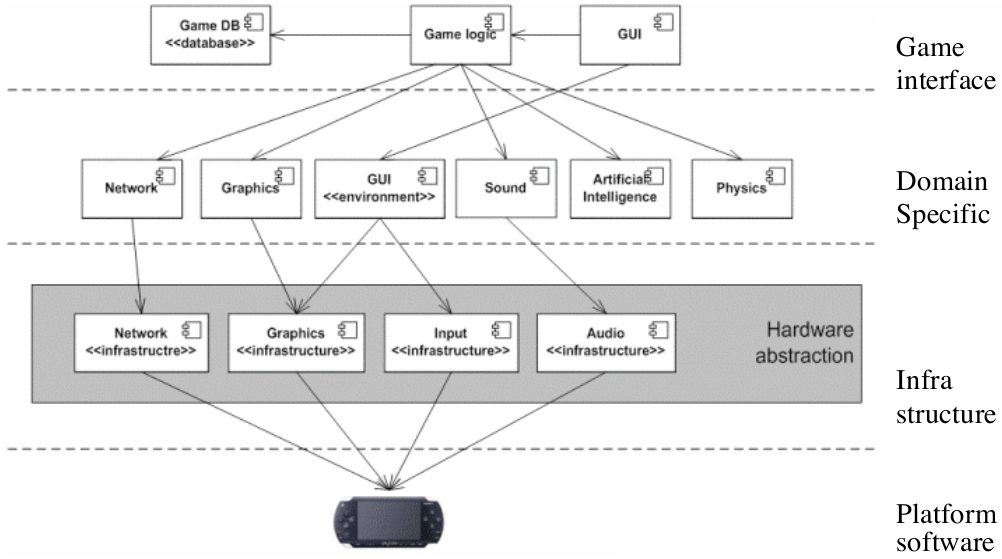
\includegraphics[scale=0.3]{pics/referencearch}
\caption{The reference architecture for games as given by Folmer -- graphic taken from the paper.}
\label{fig:referencearch}
\end{figure}

\cite{Rollings.2003} emphasizes the need for well thought-out interfaces between the components. So that for example a
route finding library/class can easily be exchanged for another one. Thus avoiding tight coupling between the high
level components where possible. He does not go into any deep details concerning components on the soft architecture
side, but he gives many ideas for design patters that can be used in game programming, such as the \textit{Singleton},
\textit{Factory} or \textit{Delegate} patters.
\linebreak

I found \citet{Fh02ageneric} particularly interesting, as it describes a system based only on components in great
detail. Haller not only explains the use of components, but also gives a very detailed proposition on how to handle
inter-component communication using a message system, based on and extending the QT GUI Framework\footnote{QT website:
\url{http://qt.nokia.com/}}.

Haller explains that components can be connected to each other using strictly typed in and outputs, making it possible to connect components
using an external (graphical) tool, easily usable by non-programmers. Having well defined in and outputs allows the
creation of component networks where as set of components are connected with each other over their in and
outputs. These networks can be looked at as a "meta-component" as the network has well defined in and outputs and can
thus itself be viewed as a component. Each component has a state in which it is in, when this state is changed a message
is sent through the outputs. The basic interface is given in \figref{fig:component}.

\begin{figure}[!htb]
\center
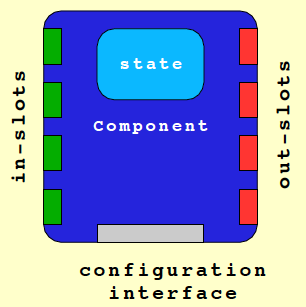
\includegraphics[scale=0.4]{pics/component}
\caption{The component interface as described by Haller \cite{Fh02ageneric} -- graphic taken from the paper.}
\label{fig:component}
\end{figure}

\cite{Doherty_2003} gives recommendations on how to structure a complete game-engine. He discusses the options of using
a component-based approach or a object-oriented design. He claimes one important advantage of using a component-based approach is:
\begin{quote}
It enforces a data-driven design philosophy. Since objects cannot be anything but data, all behavior must
be defined in terms of data. -- \cite[Page 4]{Doherty_2003}
\end{quote}
He argues this should be a favorable goal in the programming of a game, as it seperates the data from the code. By doing this it
ensures that game-designes can work in parallel with the programmers, but no recompiling of the software is needed to
change basic game attributes. Thus the teams productivity is improved.

He also brings arguments that favor the object-oriented system:
\begin{quote}
The internal representation matches the way that people think about the world. -- \cite[Page 4]{Doherty_2003}
\end{quote}

From reading his paper, I think he clearly favors the component-based approach. While acknoledging that it is more
difficult for the programmer to implement, it gives great benefitis for the game-designer. He claims that many problems
occuring with component-based systems can be solved using database proven concepts.



\subsection{Used Technology and Software}
In this section I present an overview over the technology used for this project.

\paragraph{YAML}
\begin{quote}
\textit{YAML is a human friendly data serialization standard for all programming languages.} -- \url{http://www.yaml.org}
\end{quote}
YAML has many similarities to Python, as it depends on the indention to be correct in order for the parser to work
correctly and uses a similar syntax for lists and dictionaries. This has already proven useful for the \UH{} code-base
in my experience, as all code is well formatted. These strict formatting rules should result in nicely formatted object
files and result in easier maintenance.

YAML is already being used by \UH{} to describe scenarios and campaigns, therefore it is an obvious option to use for
similar purposes.

The reason to choose YAML at the time was, that it is very easy to read and edit by humans. This comes at the cost of
being a little slower when parsing. As most data can be cached and has to be loaded from disc only once, this is not a
major concern.

\paragraph{SQLite}
\begin{quote}
\textit{SQLite is a software library that implements a self-contained, serverless, zero-configuration, transactional SQL
database engine. SQLite is the most widely deployed SQL database engine in the world. The source code for SQLite is in
the public domain.} -- \url{http://www.sqlite.org}
\end{quote}

The \UH{} project currently uses SQLite database files to store all game data, like object attributes, maps and
savegames. SQLite provides a very fast access to this data, making it a good choice where big amounts of data have to
accessed in a short amount of time -- for example map loading.

\subsubsection{Games}
In this subsection I introduce the games analyzed in this project.

\paragraph{Unknown Horizons}
\begin{quote}
\begin{center}
\includegraphics[scale=0.2]{pics/uhlogo}\end{center}
\textit{"\UH{} is a 2D realtime strategy simulation with an emphasis on economy and city building. Expand your small settlement
to a strong and wealthy colony, collect taxes and supply your inhabitants with valuable goods. Increase your power with
a well balanced economy and with strategic trade and diplomacy."} -- from \url{http://www.unknown-horizons.org}
\end{quote}

The basic game play is well known from the successful "Anno" series by Sunflowers/Ubisoft\footnote{Anno Series on
Wikipedia: \url{http://en.wikipedia.org/wiki/Category:Anno_series}}: using only few resources on a ship the player sets
out to conquer new land on an island of his choice and tries to guide his colony to wealth and power.

\UH{} has been been in active development for over four years and has been played by many thousands players from around
the world\footnote{\UH{} download statistics: \url{http://sourceforge.net/projects/unknownhorizons/files/Unknown
Horizons/}}. 

This year (2011) \UH{} participated in the \textit{Google Summer of Code} mentoring three successful students
together with its graphics engine FIFE\footnote{FIFE website: \url{http://www.fifengine.net}}, demonstrating that it has
an active community and is regarded as an important part of the \OS{} gaming world.

\paragraph{The Battle of Wesnoth}
\begin{quote}
\begin{center}
\includegraphics[scale=0.4]{pics/wesnothlogo}\end{center}
\textit{"The Battle for Wesnoth is a Free, turn-based tactical strategy game with a high fantasy theme, featuring both
single-player, and online/hotseat multiplayer combat. Fight a desperate battle to reclaim the throne of Wesnoth, or take
hand in any number of other adventures..."} -- from \url{http://www.wesnoth.org}
\end{quote}

\BOW{} is probably one of the best known and most stable \OS{} games on the market and has a huge developer community
with 103 registered developers on their GNA project page\footnote{\BOW{} gna.org page:
\url{http://gna.org/projects/wesnoth/}} and approaching ticket number 20000 on their bugtracker\footnote{\BOW{}
bugtracker: \url{http://gna.org/bugs/?group=wesnoth}}. Over 20000 members are registered at the project's forum:
\url{http://forums.wesnoth.org/}.

The first released version was 0.1 in 2003, version 1.0 was released in 2006. The current stable release 1.8.6 has over
190.000 downloads on sourceforge\footnote{\BOW{} downloads page:
\url{http://sourceforge.net/projects/wesnoth/files/wesnoth-1.8/}}. With the mature state of the project it makes for
an interesting case-study candidate.

\paragraph{MegaGlest}
\begin{quote}
\begin{center}
\includegraphics[scale=0.5]{pics/glestlogo}\end{center}
\textit{"MegaGlest is a free and open source 3D real-time strategy (RTS) game, where you control the armies of one of
seven different factions: Tech, Magic, Egyptians, Indians, Norsemen, Persian or Romans. The game is setup in one of 16
naturally looking settings, which -like the unit models- are crafted with great appreciation for detail. Additional game
data can be downloaded from within the game at no cost."} -- from \url{http://www.megaglest.org}
\end{quote}

\GLEST{} is a fork of the old project \textit{GLEST} on which development has stopped. \textit{GLEST} is now being
developed in two versions \GLEST{} and \textit{Glest Advanced Engine}. \GLEST{} is the stabler version of these two
projects which is why I chose to analyze it instead of the \textit{Glest Advanced Engine}.

\textit{GLEST} version 1.0.0 was released in 2004, the first \GLEST{} version (3.3.2) was released in
2010\footnote{\GLEST 3.3.2 release announcement: \url{http://glest.org/glest_board/index.php?topic=4917.0}}. With it's
long history \GLEST{} is a very mature game with a big community, making it a good choice for my case-study.

\paragraph{0A.D.}
\begin{quote}
\begin{center}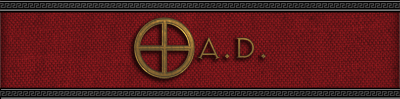
\includegraphics[scale=0.8]{pics/0ad}\end{center}
\textit{"0 A.D. (pronounced “zero ey-dee”) is a free, open-source, cross-platform real-time strategy (RTS) game of
ancient warfare. In short, it is a historically-based war/economy game that allows players to relive or rewrite the
history of Western civilizations, focusing on the years between 500 B.C. and 500 A.D. The project is highly ambitious,
involving state-of-the-art 3D graphics, detailed artwork, sound, and a flexible and powerful custom-built game engine."}
-- from \url{http://wildfiregames.com/0ad/}
\end{quote}

\AD{} started as a total conversion for \textit{Age of Empires II} by a group of friends. The team quickly moved to
their own game concept as they felt limited in their possibilities by the idea of a total conversion. The code was made
\OS{} only in 2009, the first releases followed in 2010.

The fact that the developers explicitly try to develop a engine and a game, not both in one should provide interesting
insight on the design decisions necessary when creating a game-engine.






\section{Own Contribution}

\subsection{Unknown Horizons}

\subsection{Battle of Wesnoth}

\subsection{Mega Glest}

\subsection{0 A.D.}

\subsection{Evaluation}

\subsection{Transferring the Results to Unknown Horizons}
\subsubsection{Design}
\subsubsection{Implementation}

\section{Design \& Implementation}
In this section I discuss the design of the new component system introduced into \UH{} and give details about the new
implementation.

\subsection{Design}

\subsubsection{Prerequisites}
As the code base of \UH{} is already quite big and evolved it is not possible to create a design that requires a
complete rewrite of the code or which requires all the implementation work being done in one step. Therefore I aim at
creating a design that can be implemented in smaller steps and is compatible with the current code design.

\subsubsection{Data}
A major flaw in the current \UH{} way of storing the game data is that all the game data is stored in SQLite databases,
which are difficult to edit for non-programmers. As most content contributers are not programmers, this is a major
concern. I will therefore move the data to a file based storage system, which is easily human read- and editable.

\subsubsection{Code}
To ensure compatibilty with the old inheritance based code, I will use a \textit{ComponentHolder} class, which manages all the
components an object has. This class can be included into any inheritance tree and thereby extending the current code
with the possibility of containing components. By using this approach I can slowely extract single classes from the code
and move them into components.

A component should be class to handle a specific task only and should be as independent
as possible from other components. Clearly a component can depend on other components being present, for example if I
decide to add a component that manages the production process, it will most likely depend on a component which manages
storage of items for this entity. These dependencies should be checked when the object is constructed to warn the
content creator if there are errors in this regard.
Each component has to be able to save and load its state without depending on any work being done by other components,
to ensure they are loosely coupled and easy to test.

\subsection{Implementation}
In this section I will discuss the details of the implementation.

\subsubsection{Dataformat}
\UH{} already uses YAML\footnote{YAML website: \url{http://www.yaml.org/}} to describe scenarios and campaigns. The
reason to choose YAML at the time was, that it is very easy to read and edit by humans. This comes at the cost of being
a little slower when parsing. As most data can be cached and has to be loaded from disc only once, this is not a major
concern.

I decided to use YAML for the object description files as well, the requirements match and it avoids adding another
dependency to the project. The result of converting most of the data in the database to a YAML based file for each
object looks similar as \listref{uhyaml}. It contains all basic information needed for every building and a list of components
that are used by this specific building. As the conversion from an inheritance based approach to a component based
approach is only done in small steps, we have to specify the original base class for every object using the
\textit{baseclass} attribute.


\begin{lstlisting}[language=python,caption=A basic (shortened) building definition in YAML for \UH{}, label=uhyaml]
id: 24
name: Brickyard
baseclass: production.Refiner
radius: 8
cost: 15
cost_inactive: 5
size_x: 2
size_y: 4
inhabitants_start: 1
inhabitants_max: 1
button_name: brickyard-1
tooltip_text: Turns clay into bricks.
settler_level: 1
buildingcosts: {1: 500, 4: 6, 6: 1}
components:
- HealthComponent: {maxhealth: 1000}
- ProducerComponent:
    productionlines:
      33:
        produces:
        - [7, 1]
        consumes:
        - [21, -1]
        time: 15
- StorageComponent:
    inventory:
      SlotsStorage:
        slot_sizes: {21: 4, 7: 10}
actionsets:
  as_brickyard0: {level: 0}
\end{lstlisting}

\paragraph{Loading and Caching}
As loading YAML files is too slow to be repeated for every object creation in game, the data has to be cached after
reading it once. We use the abilities of Python to create a special type instance for every object. This type instance can
than be instantiated to a "normal" python object instance. It can be thought of as creating classes on the fly. We
create a lumberjack type for example, so for every new lumberjack in the game we can create a new object instance from
this type.
Since the data from the YAML file is only read once during type creation, we efficiently cache all the data in the
type instance for later use.

\subsubsection{Code Layout}
To achive easy compatibilty with the old inheritance based approach, a \textit{ComponentHolder} class has been
introduced, that manages a set of components. This class can be included into the normal hierarchy of any in-game object.

\paragraph{ComponentHolder}
The \textit{ComponentHolder} has a very basic interface:
\begin{itemize}
    \item initialize()
    \item add\_component()
    \item has\_component()
    \item get\_component()
    \item remove\_component()
    \item save()/load()/remove()
\end{itemize}
The add/has/get\_component() methods are pretty clear, they add \textit{Component}s to the \textit{ComponentHolder}, check if
they are available for this \textit{ComponentHolder} or return a specified \textit{Component}.

It is note-worthy that the \textit{ComponentHolder} contains an extra \textit{initialize()} method, which is separate from the
normal constructor. This method has to be called after instance creation on any class that inherits from the
\textit{ComponentHolder} class. This is a work-around for the problem that certain attributes, such as the game-engine's
visual instance, needed in the components are only ready after the entire constructor hierarchy has been executed to the
top. This will hopefully be repaired after everything has been moved to components, but for the moment this is a
necessary evil.

\paragraph{Component}
To represent a component the \textit{Component} class has been created. Each component should take care of a certain set
of functionality, which should be as independent as possible from any other code. Of course this is not always
achievable, as it soon becomes clear that special components will rely on the existence of other components. For example
a production component might rely on the presence of a storage component, with which it can work.

Each \textit{Component} has to implement the basic interface:
\begin{itemize}
    \item initialize()
    \item load()/save()
    \item remove()
    \item get\_instance() - Classmethode
\end{itemize}
As with the \textit{ComponentHolder} the \textit{Component} has to implement an \textit{initialize()} method, in which
all the setup should be done. This method is called automatically by the \textit{ComponentHolder}, so no special care
has to be taken here.

The \textit{load()}/\textit{save()} methods are called by the \textit{ComponentHolder} and should
implement loading and saving the components state into the given database. This should be done in a way, that the
component does not relay on any other part of the code to correctly restore its state on loading.

The \textit{get\_instance()} method is a class method, its purpose is to return an instance of the component, given data loaded
from the yaml file. For basic components the basic implementation is likely to suffice, it will pass in the dict of data
loaded from yaml as arguments to the class. For more sophisticated components this method might need to be
reimplemented. An example of this is the \textit{StorageComponent}.

Each component has to set the class's \textit{NAME} variable to unique string. Components that inherit from other
components can usually keep the name of the inherited class, as they are not used in the same \textit{ComponentHolder}
instance. Keeping the name the same, also ensures that if they implement similar functionality it is possible to call
\textit{get\_component()} with the parent class, and still receiving the correct implementation. This is used for example
for names. A \textit{NamedComponent} has been implemented. It handles giving names to objects. There are some special
implementations of this, for example the \textit{ShipNameComponent}, which uses special names designated for ships. If a
\textit{ShipNameComponent} component is present in the \textit{ComponentHolder} class and get\_component{NamedComponent}
is called, the \textit{ShipNameComponent} is returned, as they both use the same \textit{NAME} variable.

\subparagraph{Dependencies}
\textit{Components} can depend on other components to exist. For this every \textit{Component} class can use the
\textit{DEPENDENCIES} class variable. It is a list of \textit{Component} classes. The classes specified will be
initialized before the class that lists them as dependencies. 

The basic dependency resolution is done by implementing the \textit{\_\_lt\_\_()} (less than) method on the Component,
so that a list of \textit{Components} can be sorted by dependency order. This is of course a very basic form of
dependency resolution, which can't detect circular dependencies, etc. It should be good enough for this purpose and is very
simple and fast, as it uses python built-in \textit{sorted()} method.


\subsection{Added Components}
Since the scope of the project is not big enough turn the \UH{} codebase into a completely component driven
architecture, only parts of the classes have been converted to \textit{Component}s yet. The following \textit{Component}
implementations have been made:
\begin{itemize}
    \item AmbientSoundComponent
    \item HealthComponent
    \item NamedComponent + Subclasses
    \item StanceComponent
    \item StorageComponent
    \item TradePostComponent
    \item Producer
\end{itemize}

\paragraph{AmbientSoundComponent}
The \textit{AmbientSoundComponent} takes care of playing sounds in-game. It can position sounds at the current position
of an entity and saves a list of all the sounds an entity can play. The goal of this component is to collect all sound
handling code in one place. Since we do not have a lot of this code, this component was a good start together with the
\textit{NamedComponent}.

\paragraph{HealthComponent}
Together with the \textit{StanceComponent} this was one of the components that had been created during the project's
participation in \textit{Google Summer of Code 2011}. This was the first try of working on a component based system. I
did not make major changes to this component, other than fitting it into the new interface.

Its purpose is to provide a health counter for objects and handle everything that is connected with this, like drawing
life-bars.

\paragraph{NamedComponent + Subclasses}
The \textit{NamedComponent} provides unique names for an object throughout one game. For this class several subclasses
exist, that provide different names. Namely these are:
\begin{itemize}
    \item \textit{ShipNameComponent}
    \item \textit{PirateShipNameComponent}
    \item \textit{SettlementNameComponent}
\end{itemize}

\paragraph{StanceComponent}
The \textit{StanceComponent} is used to set the combat stance of the object. It can be aggresive, defensive or neutral.
This Component was introduced during the \textit{Google Summer of Code 2011} as part of the combat system
implementation.

\paragraph{StorageComponent}
The \textit{StorageComponent} provides the entity with a sort of inventory where it can store different resources. This
is a fairly complex component, as it can use different storage implementations internally. For this reason this
component has to implement its own \textit{get\_instance()} method. An example markup for the \textit{StorageComponent}
using an inventory that can handle a fixed set of slots with specific sizes is given in \figref{storagyaml}.

\begin{lstlisting}[language=python,caption=YAML representation of the StorageComponent using a SlotStorage,
label=storagyaml]
- StorageComponent:
    inventory:
      SlotsStorage:
        slot_sizes: {28: 8, 5: 8}
\end{lstlisting}

\paragraph{TradePostComponent}
The \textit{TradePostComponent} adds trading functionality to the entity. This component handles selling and buying
resources from other players or the Free-Trader.

\paragraph{Producer}
This is most complex component in the game so far and I estimate it to stay this way, even if more components are added.
It manages the production of goods in the game, but using production lines. Since this is a very complex system it is
very bug-prone and extracting it into a single component and thereby removing it from the main hierarchy of buildings
was not easy. The code depended heavily on other classes being in the inheritance tree and debugging this was very
difficult and time-consuming.

The \textit{Producer} component greatly eases the changing and adjusting of production lines for the content creator, as
all information is now at one place. Using the old SQLite system, the content creator had to look at countless tables to
be able to get an overview of even a single production line. This has greatly improved. \listref{produceryaml} provides a short
example.

\begin{lstlisting}[language=python,caption=YAML representation of the Producer with two production lines,
label=produceryaml]
- ProducerComponent:
    productionlines:
      7:
        produces:
        - [10, 1]
        consumes:
        - [2, -1]
        time: 1
      47:
        produces:
        - [31, 1]
        consumes:
        - [30, -1]
        time: 1
\end{lstlisting}

\subsection{Testing}
To ensure working code, three types of tests were used:
\begin{enumerate}
    \item Unit Test
    \item System Test
    \item Smoke Test
\end{enumerate}

\paragraph{Unit and System Tests}
\UH{} has a set of unit and system tests. Unit tests are basic tests for single classes to check their functionality.
System tests try to test the working of the entire game, instead of just a small function. It has a more general scope
to discover bugs in game logic.
After making the changes to the code, all tests have been repaired to work as expected. Also a few tests concerning the
new component system have been added. Together with the community I am working on extending the tests to cover more code
and to make sure my changes are stable before they are merged into the mainline of development.

\paragraph{Smoketests}
A smoke test describes a kind of test in which the goal is to run as much code of the system as possible and see if it
fails \cite{Mcconnell:1996:DBS:624614.625626}.

To emulate this, I used our artificial intelligence player. I started the game on 20 times the normal speed and
let 3 AI players play for a while. This helped me find a lot of bugs, especially in the beginning. As python is not
strictly typed, the interpreter discovers a lot of bugs, like missing attributes, only at runtime. Therefore it is
crucial to acutally run as much game code as possible.

\section{Evaluation}
In this section I will evaluate the project and the result.

\subsection{Project}
The project was executed in an autonomous way, without much interaction of the professor or other mentors. The focus was
on mainly working with other people involved in \UH{} or other \OS{} games discussed in this work. This way it has a
direct impact on the work of \UH{} and might have lead to some additional insights for members of other teams.

I believe the result matches the style of project execution, it had more emphasis on implementing the new
system than production many pages of documentation. A lot of time has been invested to implement a stable system that can be used in the
production mainline of development in \UH{}.

The plans for the implementation were worked on and discussed with the \UH{} team throughout the project and during the
weekly meetings\footnote{Meeting logs:
\url{http://meetings.christoph-egger.org/unknown-horizons/2011/unknown-horizons.2011-10-16-17.02.html}}\footnote{Meeting
logs 2: \url{http://meetings.christoph-egger.org/unknown-horizons/2011/unknown-horizons.2011-12-04-17.04.html}}. This
allowed me to identify weeknesses in my design and ensure that I have the same ideas, of how it should look, as the rest
of the team.

\subsection{Results}
This project provides two main results:
\begin{enumerate}
    \item Case-study of four existing systems to describe in-game entities
    \item Implementation of a new component system for \UH
\end{enumerate}

\paragraph{Case Study}
In the case study I have explained how the four project \UH{}, \BOW{}, \GLEST{} and \AD{} represent their objects as
in dataformat as well as in code. It provides insight for new projects on how a component based system can be designed
and on the quality of code-architecture in \OS{} games.

While the last part has not been explicitly discussed, it is clear that some thought on how to design these systems is
being put into the systems. Especially \AD{} provides a very cleanly designed system, designed for ease of development
and content creation with a very clear code structure.
It provides a purely component based system, making it the best designed of the four discussed projects under this point
of research.

\paragraph{Implementation}
The first lesson learned from this project is that refactoring the entire code of \UH{} to component based system is a
lot of work, that if persued further will require enourmous effort on the side of the developer team. Since it provides
great benefits to the code-quality, as in less coupling and thus better testability, it is likely that more work in this
area will be done.

The implementation allows for an easier representation of entities outside the code, making it very interesting
for content creators, as they can now change the game behaviour of entities in an easy way -- by just using a simple
text-editor.


\subsection{Methods}

\section{Conclusion and Future Work}
In this section I present a conclusion of this project and the future work that can follow it.

\subsection{Conclusion}



\subsection{Future Work}




%\appendix

%\chapter{Patches}\label{appendix}


\chapter{Grammars}\label{appendixGrammars}


%\bibliography{references}

\end{document}
